\chapter{量子力学的实验起源}\label{chap:experimental-origins}

量子力学以其有争议的概率性质以及波和粒子的奇特结合而著称,是一套非常奇怪的理论.它并不是因为有人认为世界本来就应该这样运行才被发明出来的,而是因为各种实验表明:不管人们是否喜欢,世界确实就是这样运行的.Fermilab 粒子天体物理学中心主任 Craig Hogan 曾这样说:

\begin{quote}
如果不是数据逼着我们这样做,任何头脑正常的理论家都不会发明量子力学.\footnote{引自 Michael Moyer 的文章 ``Is Space Digital?'',载于 \textit{Scientific American},2012 年 2 月,第 30--36 页.}
\end{quote}

量子力学最初的曙光出现在 1900 年,当时 Planck 解决了黑体辐射问题;但完整的理论直到 1925--1926 年才出现,其标志是 Heisenberg 的矩阵模型、Schrödinger 的波模型,以及 Born 对波模型的统计解释.

\section{光是波还是粒子？}\label{sec:light-wave-or-particle}

\subsection{Newton 与 Huygens}\label{subsec:newton-huygens}

从 17 世纪末一直到 18 世纪初,科学界围绕光的本质展开了激烈争论.一派追随 Isaac Newton 的观点,认为光由一群粒子或“微粒”组成;另一派则由荷兰物理学家 Christiaan Huygens 领导,认为光是一种波.Newton 认为,只有微粒理论才能解释光倾向于沿直线传播这一观察事实.另一方面,Huygens 等人认为,波动理论能够解释光的许多已知现象,包括光从一种介质进入另一种介质时发生的弯曲,即光的“折射”,例如从空气进入水中时的情形.Newton 的声望如此之高,以至于他的“微粒”理论一直占据主导地位,直到 19 世纪初才逐渐改变.

\subsection{光的波动理论的兴起}\label{subsec:wave-theory-light}

1804 年,Thomas Young 发表了两篇论文,描述并解释了他的双缝实验.在这个实验中,阳光先通过纸板上的一个小孔,再照射到另一块带有两个小孔的纸板上,随后光线照到第三块纸板上,在那里可以观察到光形成的图样.Young 观察到光的“条纹”,即明暗交替的区域.他认为光是一种波,并提出这些条纹是从两个小孔发出的波相互干涉的结果.

Young 把光与水作了类比,因为水波的干涉很容易观察到.如果两列圆形水波彼此交叉,就会有一些点恰好是一列波的波峰与另一列波的波谷相遇,从而产生相消干涉,也就是两列波部分抵消,使合成波在该点的振幅变小.另一方面,在另一些点,一列波的波峰会与另一列波的波峰重合,或者一个波谷与另一个波谷重合.在这些点,会产生相长干涉,使合成波的振幅变大.相长干涉与相消干涉交替出现,就会在合成波中形成类似棋盘格的图样:振幅大和振幅小的区域交替排列.每个区域的尺度大致与单个波的波长同阶.

借助水波的这个类比,Young 解释了自己观察到的干涉条纹,并预测了要形成所观察到的具体图样,光必须具有怎样的波长.根据观察,Young 认为可见光的波长从光谱红端的大约 $1/36{,}000$ 英寸(约 $700\,\mathrm{nm}$)到紫端的大约 $1/60{,}000$ 英寸(约 $425\,\mathrm{nm}$),这一结果与现代测量相符.

图~\ref{fig:interference-waves} 展示了从两个不同点发出的圆形波如何形成干涉图样.可以把 Young 实验中的第二块纸板想象成位于图的上方,两个小孔靠近左上方和右上方.图~\ref{fig:intensity-plot} 则绘出了强度(即位移的平方)关于 $x$ 的函数图像,其中 $y$ 取图~\ref{fig:interference-waves} 底部所对应的值.

\begin{figure}[htbp]
  \centering
  \includegraphics[page=20,pagebox=cropbox,trim=79.28bp 416.15bp 88.08bp 66.56bp,clip,width=.72\linewidth]{../input/source/Quantum Theory for Mathematicians(Brian C. Hall).pdf}
  \caption{从两个狭缝发出的波的干涉.}\label{fig:interference-waves}
\end{figure}

\begin{figure}[htbp]
  \centering
  \includegraphics[page=21,pagebox=cropbox,trim=115.28bp 477.36bp 124.08bp 66.87bp,clip,width=.78\linewidth]{../input/source/Quantum Theory for Mathematicians(Brian C. Hall).pdf}
  \caption{沿图~\ref{fig:interference-waves} 底部水平线得到的强度图.}\label{fig:intensity-plot}
\end{figure}

尽管 Young 的实验具有令人信服的力量,许多光的微粒理论支持者仍然没有被说服.1818 年,法国科学院举办了一场论文竞赛,要求解释光的已知性质.参赛论文之一是 Augustin-Jean Fresnel 的文章,他在其中进一步阐述了 Huygens 的折射波动模型.微粒理论的支持者 Simeon-Denis Poisson 读到 Fresnel 的论文后,嘲笑这一理论,指出如果该理论正确,经过不透明圆盘旁边的光就会在圆盘边缘发生衍射,并在圆盘阴影的中心形成一个亮斑;Poisson 认为这种预言荒谬.然而,竞赛评审委员会主席 Francois Arago 决定用实验检验这一问题,结果发现这样的亮斑确实会出现.这个亮斑通常被称为“Arago 斑”,有时甚至带有讽刺意味地称为“Poisson 斑”.后来 Arago 意识到,这个亮斑其实早在一百年前就已经由 Delisle 和 Maraldi 在各自的实验中观察到.

Arago 对 Poisson 斑的观察使光的波动理论得到广泛接受.1865 年,James Clerk Maxwell 整理出了今天所称的 Maxwell 方程,这一理论获得了更大的支持.Maxwell 证明,他的方程预言电磁波会以某个速度传播,而这个速度与观察到的光速一致.因此 Maxwell 得出结论:光就是一种电磁波.从 1865 年直到 19 世纪末,关于光究竟是波还是粒子的争论被认为已经彻底解决,结论倾向于波动理论.

\subsection{黑体辐射}\label{subsec:blackbody-radiation}

进入 20 世纪初,光的波动理论开始面临新的挑战.第一个挑战来自黑体辐射理论.在物理学中,黑体是一个理想化物体,它能够完全吸收照射到其上的一切电磁辐射.在现实世界中,可以用表面具有高度吸收性的物体(例如“灯黑”)近似黑体.黑体辐射问题研究的是黑体内部空腔中的电磁辐射分布.虽然黑体壁会吸收照射到其上的辐射,但构成黑体壁的原子发生热振动,会使黑体发出电磁辐射.(在通常温度下,发出的辐射大多处在红外波段.)

因此,在空腔中,电磁辐射会不断被吸收和重新发射,直到达到热平衡;此时,在每个频率上,辐射的吸收与发射恰好平衡.根据(经典)统计力学的“能量均分定理”,电磁辐射任意给定模式中的能量应当服从指数分布,其平均值为 $k_B T$,其中 $T$ 是温度,$k_B$ 是 Boltzmann 常数.(温度应当用这样一种标度来测量:绝对零度对应于 $T=0$.)这个预言的困难在于,每个模式的平均能量都相同(这正是“能量均分”这一术语的来源).于是,把所有模式加起来--而模式有无穷多个--就会得到空腔内的能量为无穷大.这一奇怪的预言被称为紫外灾难,因为无穷大的能量来自光谱的紫外(高频)端.紫外灾难在物理上似乎没有意义,当然也与真实黑体中观察到的能谱不相符.

Max Planck 在 1900 年发表的一篇论文中给出了黑体能谱的另一种预言.Planck 假设,在给定频率 $\omega$ 下,电磁场的能量应当是“量子化”的,也就是说,这个能量只能取某个基本单位的整数倍,这个基本单位等于 $\hbar\omega$,其中 $\hbar$ 是一个常数,即我们现在所称的 Planck 常数.Planck 认为,能量仍然会服从指数分布,但只在 $\hbar\omega$ 的整数倍上取值.在低频率下,Planck 理论与经典统计力学的预言基本相同;在高频率下,即 $\hbar\omega$ 与 $k_B T$ 相比很大时,Planck 理论预言平均能量会迅速下降(具体细节见练习~\ref{ex:planck-mean-energy}).事实上,如果分别以克、厘米和秒作为质量、距离和时间的单位,并把 $\hbar$ 的数值取为

\begin{equation}
  \hbar=1.054\times 10^{-27},\label{eq:planck-constant-cgs}
\end{equation}

那么 Planck 的预言就与实验观察到的黑体能谱相符.

Planck 把黑体壁想象成由不同频率的相互独立的振子组成,并假设每个振子的能量只能取 $\hbar\omega$ 的整数倍.这个图像显然并不是对黑体中电磁能量为何量子化的现实物理解释,但它暗示 Planck 认为能量量子化源于空腔壁的性质,而不是电磁辐射本身的内在性质.另一方面,Einstein 在评估 Planck 的模型时认为,能量量子化是辐射本身固有的.在 Einstein 的图像中,给定频率的电磁能量--无论处在黑体空腔中还是其他地方--都以能量与频率成正比的包或量子的形式出现.每一个电磁能量量子就是我们现在所称的一个光子,可以把它看作一个光粒子.因此,Planck 的黑体辐射模型重新开启了光的粒子理论.

顺带一提,1900 年也正是 Planck 的黑体辐射论文发表的那一年,Lord Kelvin 发表了一次演讲,提醒人们注意经典统计力学理论的另一个困难.Kelvin 把 19 世纪物理学在 20 世纪初所面临的困难描述为两朵“乌云”.第一朵乌云与以太有关--以太是一种假想介质,电磁辐射通过它传播;Michelson 和 Morley 试图观察地球相对于以太的运动,却没有成功.在这朵乌云下面,隐藏着狭义相对论.Kelvin 所说的第二朵乌云与气体的热容量有关.经典统计力学的能量均分定理对定压热容 $c_p$ 与定容热容 $c_v$ 之比作出了预言,而这个预言与实验测得的比值有很大偏差.在第二朵乌云下面,隐藏着量子力学,因为解决这一差异的方式与 Planck 解决黑体问题的方式相似:量子力学对能量均分定理作出了修正,从而改变了 $c_p$ 与 $c_v$ 之比的预言,使其能够与观察到的比值相符.

\subsection{光电效应}\label{subsec:photoelectric-effect}

1905 年是 Einstein 的 annus mirabilis(奇迹年):这一年 Einstein 发表了四篇划时代的论文,其中两篇关于狭义相对论,另外两篇分别关于 Brown 运动和光电效应.Einstein 因光电效应于 1921 年获得诺贝尔物理学奖.在光电效应中,照射到金属上的电磁辐射会使电子从金属中逸出.Einstein 发现,增大入射光的强度时,逸出电子的数目会增加,但每个电子的能量并不改变.

从光的波动理论角度看,这个结果很难解释.毕竟,如果光只是一种电磁波,那么增大光强就相当于增大相应电场和磁场的强度;而场强增强又应该增加传递给电子的能量.

另一方面,光的粒子理论可以很自然地解释 Einstein 的结果.假设光实际上是一股粒子流(光子),每个粒子的能量由其频率决定.那么,对于给定频率的光,增大光强只会增加光子的数目,不会影响每个光子的能量.如果每个光子都有一定概率撞击电子并使其逃离金属,那么逸出电子的能量就由入射光的频率决定,而不由入射光的强度决定.因此,光电效应为相信光能够以粒子方式表现提供了又一个有力理由.

\subsection{重新审视双缝实验}\label{subsec:double-slit-revisited}

虽然 Planck 和 Einstein 的工作揭示了光的粒子性,但 Young、Arago 和 Maxwell 等人的工作也清楚表明光具有波动性.因此,光必定在某些情况下表现得像波,在另一些情况下表现得像粒子;这种现象被称为“波粒二象性”.William Lawrence Bragg 曾这样描述这一情形:

\begin{quote}
上帝在星期一、星期三和星期五按照波动理论运行电磁学;魔鬼则在星期二、星期四和星期六按照量子理论运行电磁学.
\end{quote}

(显然,星期日是休息日,不必加以解释.)

我们已经看到,19 世纪初的 Young 双缝实验是支持光的波动理论的一条重要证据.如果光确实由粒子组成,而黑体辐射和光电效应都指向这一点,那么就必须用基于粒子的方式解释双缝实验.J. J. Thomson 在 1907 年提出,双缝实验中观察到的光图样可能来自不同光子之间某种形式的相互干涉.于是 Thomson 推测,如果光强足够低,光子之间会相距很远,干涉图样也许就会消失.1909 年,Geoffrey Ingram Taylor 试图检验这一推测,结果发现,即使把光强大幅降低(低到形成其中一幅图像需要三个月),干涉图样仍然保持不变.

既然 Taylor 的结果表明,即使光子相距很远,干涉仍然存在,那么光子就不是彼此干涉的.正如 Paul Dirac 在 [6] 第 1 章中所说:“每一个光子只与它自己发生干涉.”换一种说法,由于只有一条狭缝时没有干涉,Taylor 的结果表明,每个光子都通过了两条狭缝.到了 20 世纪 60 年代初,人们已经能够用电子而不是光子进行双缝实验,由此获得了更生动的量子物质奇异行为的证据(见第~\ref{sec:electron-wave-particle} 节).

\section{电子是波还是粒子？}\label{sec:electron-wave-particle}

20 世纪初,物质的原子理论已经牢固建立.Einstein 关于 Brown 运动的 1905 年论文是对该理论的重要确认,并且给出了用日常单位计算原子质量的第一个方法.1909 年,Hans Geiger 和 Ernest Marsden 在 Ernest Rutherford 指导下进行的实验,使 Rutherford 在 1911 年提出了这样一种原子图像:原子的大部分质量集中在一个很小的原子核中.在 Rutherford 模型中,每个原子都有一个带正电的原子核,其电荷为 $nq$,其中 $n$ 是正整数,即原子序数,而 $q$ 是电荷的基本单位,最早在 Millikan 著名的油滴实验中被观察到.原子核周围是由 $n$ 个电子组成的云,每个电子带负电 $-q$.当原子结合成分子时,一个原子的某些电子可能与另一个原子共享,从而在原子之间形成化学键.这种原子及其成键的图像引出了现代化学理论.

原子理论的基础之一是把电子看作粒子;事实上,每个原子中的电子数就被定义为其原子序数.然而,物质的原子理论得到确认后不久,人们就开始观察到电子的波动性质.电子的情形与光恰好相反:光长期被认为是波(至少从 Maxwell 方程在 1865 年发表起,一直到 Planck 在 1900 年的工作为止),后来才发现它具有类似粒子的行为;电子最初被认为是粒子,后来才发现它具有类似波的性质.但最终,光和电子都同时具有波动性和粒子性.

\subsection{氢的谱}\label{subsec:hydrogen-spectrum}

如果让电流通过一个装有氢气的管子,气体就会发光.用棱镜把这束光分解成不同频率后,会显现出一条条谱带,这说明光并不是许多不同频率的连续混合,而只包含一族离散的频率.根据光的光子理论,每个光子的能量与其频率成正比.因此,每个观察到的频率都对应于氢原子向电磁场转移的一定能量.

氢原子由一个质子和一个电子组成.由于质子的质量远大于电子,可以把质子看作静止不动,而电子绕着质子运动.于是,电流通过气体时,电子会被激发到较高能量状态;最终,电子会回到较低能量状态,同时发射一个光子.这样,通过观察所发射光子的能量(或者等价地,频率),就可以反推出电子能量的变化.

上一段描述中的奇怪之处在于:所发射光子的能量--因而电子的能量--只取一族离散的可能值.根据观察到的频率,Johannes Rydberg 在 1888 年得出电子可能具有如下形式的能量:

\begin{equation}
  E_n=-\frac{R}{n^2},\label{eq:rydberg-energy}
\end{equation}

其中 $R$ 是“Rydberg 常数”,在“Gaussian 单位制”中给出为

\begin{equation}
  R=\frac{m_e Q^4}{2\hbar^2},\label{eq:rydberg-constant}
\end{equation}

这里 $Q$ 是电子的电荷,$m_e$ 是电子的质量.(严格说来,$m_e$ 应当替换为质子--电子系统的约化质量 $\mu$,即
\[
  \mu=\frac{m_e m_p}{m_e+m_p},
\]
其中 $m_p$ 是质子的质量.不过,由于质子质量远大于电子质量,$\mu$ 几乎等于 $m_e$,因此我们忽略二者的差别.)式~\eqref{eq:rydberg-energy} 与实验相符,因为氢中观察到的所有频率(至少在 Rydberg 当时所能达到的精度下)都具有如下形式:

\begin{equation}
  \omega=\frac{1}{\hbar}(E_n-E_m),\qquad n>m.\label{eq:hydrogen-frequency}
\end{equation}

应当指出,Johann Balmer 早在 1885 年就观察到了同样形式的频率,但他只考虑了 $m=2$ 的情形,而且 Balmer 的工作对 Rydberg 产生了影响.

式~\eqref{eq:hydrogen-frequency} 中的频率被称为氢的谱.Balmer 和 Rydberg 只是在试图寻找一个能与氢中观察到的频率相匹配的简单公式.他们都没有理论解释为什么只会出现这些特定频率.这个解释要等到 20 世纪量子理论开始出现之后才会到来.

\subsection{氢原子的 Bohr--de Broglie 模型}\label{subsec:bohr-debroglie}

1913 年,Niels Bohr 提出了氢原子模型,试图解释氢的观测谱.Bohr 把氢原子想象成一个电子绕着带正电的原子核运行,这与行星绕太阳运行非常相似.经典地,质子对电子施加的力满足如下形式的平方反比定律:

\begin{equation}
  F=\frac{Q^2}{r^2},\label{eq:coulomb-force}
\end{equation}

其中 $Q$ 是电子的电荷,单位取适当的形式.

如果电子沿圆轨道运动,那么它在轨道平面内的轨迹为
\[
  (x(t),y(t))=(r\cos(\omega t),r\sin(\omega t)).
\]
对时间求二阶导数,得到加速度向量 $a$:
\[
  a(t)=(-\omega^2r\cos(\omega t),-\omega^2r\sin(\omega t)),
\]
因此加速度向量的大小为 $\omega^2r$.Newton 第二定律 $F=ma$ 要求
\[
  m_e\omega^2r=\frac{Q^2}{r^2},
\]
从而
\begin{equation}
  \omega=\sqrt{\frac{Q^2}{m_e r^3}}.\label{eq:bohr-orbit-frequency}
\end{equation}

由频率公式可以算出动量(质量乘速度)的大小:
\begin{equation}
  p=\sqrt{\frac{m_eQ^2}{r}}.\label{eq:bohr-momentum}
\end{equation}

我们还可以计算角动量 $J$.对于圆轨道,角动量就是动量乘以到原子核的距离,因此
\begin{equation}
  J=\sqrt{m_eQ^2r}.\label{eq:bohr-angular-momentum}
\end{equation}

Bohr 假设电子服从经典力学,\textit{但}其角动量是“量子化”的.具体地说,在 Bohr 模型中,角动量必须是 $\hbar$(Planck 常数)的整数倍.令 $J=n\hbar$,得到
\begin{equation}
  r_n=\frac{n^2\hbar^2}{m_eQ^2}.\label{eq:bohr-radii}
\end{equation}

如果计算半径为 $r_n$ 的轨道能量,就会发现(见练习~\ref{ex:bohr-energy})它与式~\eqref{eq:rydberg-energy} 中的 Rydberg 能量完全一致.Bohr 进一步假设,电子可以从一个允许状态跃迁到另一个允许状态,并在这个过程中发射一个频率由式~\eqref{eq:hydrogen-frequency} 给出的光量子.

Bohr 没有解释电子的角动量为什么会量子化,也没有解释电子如何从一个允许轨道运动到另一个允许轨道.因此,他的原子行为理论显然还不完整;它属于“旧量子力学”,后来被 Heisenberg 的矩阵模型和 Schrödinger 的波模型所取代.尽管如此,Bohr 模型仍然是理解原子行为过程中的重要一步,Bohr 也因这项工作获得了 1922 年诺贝尔物理学奖.Bohr 的方法仍有一部分留存在现代量子理论中:在 WKB 近似中,Bohr--Sommerfeld 条件为一维量子系统的能级给出近似(见第 15 章).

1924 年,Louis de Broglie 把 Bohr 关于角动量的条件重新解释为一个波动条件.de Broglie 假设电子可以用一个波来描述,波的空间频率 $k$ 与电子动量满足关系
\begin{equation}
  p=\hbar k.\label{eq:de-broglie}
\end{equation}

这里,“频率”的定义是:函数 $\cos(kx)$ 的频率为 $k$.这是“角频率”,与每单位距离的周期数频率相差一个 $2\pi$ 的因子.因此,与频率 $k$ 相应的周期为 $2\pi/k$.

在 de Broglie 的方法中,我们要想象有一个波叠加在电子的经典轨道上,并要求波绕轨道一周后与自身相匹配.这个条件意味着轨道应当由波的整数个周期组成:
\begin{equation}
  2\pi r=n\frac{2\pi}{k}.\label{eq:de-broglie-orbit}
\end{equation}

结合式~\eqref{eq:de-broglie} 和关于 $p$ 的式~\eqref{eq:bohr-momentum},得到
\[
  2\pi r=n\frac{2\pi\hbar}{p}=2\pi n\hbar\sqrt{\frac{r}{m_eQ^2}}.
\]
解这个关于 $r$ 的方程,恰好得到式~\eqref{eq:bohr-radii} 中的 Bohr 半径.

因此,de Broglie 的波假设为 Bohr 对角动量的量子化提供了另一种解释,并说明了氢原子允许能量的来源.当然,如果接受电子的 de Broglie 波假设,就应当预期在氢原子之外的其他情形中也能观察到电子的波动行为,而这一预期很快就会得到验证.图~\ref{fig:bohr-radii} 展示了前 10 个 Bohr 半径,其中在第 8 个和第 10 个半径上叠加画出了 de Broglie 波.

\begin{figure}[htbp]
  \centering
  \includegraphics[page=28,pagebox=cropbox,trim=115.28bp 408.11bp 124.08bp 66.49bp,clip,width=.68\linewidth]{../input/source/Quantum Theory for Mathematicians(Brian C. Hall).pdf}
  \caption{$n=1$ 到 $n=10$ 的 Bohr 半径,并在 $n=8$ 和 $n=10$ 的轨道上叠加 de Broglie 波.}\label{fig:bohr-radii}
\end{figure}

\subsection{电子衍射}\label{subsec:electron-diffraction}

1925 年,Clinton Davisson 和 Lester Germer 通过用低能电子轰击镍薄膜,研究镍的性质.由于设备出现问题,镍样品意外地被加热到很高的温度.镍冷却后形成了大块晶体,而不是原样品中的小晶体.重结晶以后,Davisson 和 Germer 观察到电子从镍样品反射时形成了原来没有出现的峰.他们一时无法解释这种图样,直到 1926 年 Davisson 了解到 de Broglie 假设,才怀疑自己观察到了 de Broglie 预言的电子波动行为.

意识到这一点后,Davisson 和 Germer 开始系统地寻找实验中的波动峰.具体来说,他们试图证明电子反射角的图样与 X 射线衍射中看到的图样相匹配.经过许多次额外测量,他们发现电子图样与 X 射线衍射图样之间存在非常接近的对应关系.由于当时人们已经知道 X 射线是电磁辐射的波,Davisson--Germer 实验有力地确认了 de Broglie 关于电子的波动图像.Davisson 和 Germer 在 1927 年发表了两篇论文;1937 年,Davisson 与 George Paget 共同获得诺贝尔物理学奖,后者在 Davisson 和 Germer 之后不久也观察到了电子衍射.

\subsection{电子的双缝实验}\label{subsec:electron-double-slit}

虽然量子理论清楚地预言,通过双缝的电子会产生与光所观察到的类似干涉,但直到 1961 年 Clauss Jönsson 的工作,这一预言才得到实验确认.主要困难在于,对于合理的能量,电子的波长远小于可见光的波长.例如,Jönsson 所使用的电子的 de Broglie 波长为 $5\,\mathrm{nm}$,而可见光的波长大约为 $500\,\mathrm{nm}$(取决于颜色).

1989 年发表的结果中,由 Akira Tonomura 领导的 Hitachi 团队完成了一次双缝实验,能够逐个记录电子的结果.(1974 年,Bologna 的 Pier Giorgio Merli、GianFranco Missiroli 和 Giulio Pozzi 也完成了类似但不那么明确的实验,并于 1976 年发表在 \textit{American Journal of Physics} 上.)在 Hitachi 实验中,每个电子通过狭缝后撞击屏幕,使一个小光点出现;随后逐个记录每个电子所产生的光点位置.关键在于,每个电子都只在一个点撞击屏幕.也就是说,单个电子并没有像波那样在整个屏幕上铺开,而是表现得像点粒子,因为观测到的电子位置确实是一个点.然而,每个电子撞击的位置都不同;当大量电子撞击并记录它们的位置后,就会出现干涉图样.

电子位置的变化本身并不令人惊讶,因为可以用电子射向狭缝的方式存在微小差异来解释这种变化.真正令人惊讶的是具有鲜明特征的干涉图样:在很短的距离内,电子撞击的图样快速变化,其中包括几乎没有电子撞击的区域.(把图~\ref{fig:electron-interference} 与图~\ref{fig:intensity-plot} 比较.)还要注意,在实验中电子彼此相距很远,因此装置中任何时候都不会有超过一个电子.于是,电子不可能彼此干涉;相反,每个电子都与自己发生干涉.图~\ref{fig:electron-interference} 展示了 Hitachi 实验的结果,其中观察到的电子数从第一幅图中的约 150 个逐渐增加到最后一幅图中的 160,000 个.

\begin{figure}[htbp]
  \centering
  \includegraphics[page=30,pagebox=cropbox,trim=53.24bp 406.19bp 62.76bp 66.92bp,clip,width=.82\linewidth]{../input/source/Quantum Theory for Mathematicians(Brian C. Hall).pdf}
  \caption{1989 年 Hitachi 实验中的四幅图像:单个电子的撞击逐渐累积形成干涉图样.图像来自 Akira Tonomura 和 Wikimedia Commons 用户 Belsazar,采用 Creative Commons Attribution-Share Alike 3.0 Unported 许可.}\label{fig:electron-interference}
\end{figure}

\section{Schrödinger 与 Heisenberg}\label{sec:schrodinger-heisenberg}

1925 年,Werner Heisenberg 提出了一个量子力学模型,基本思想是把粒子的位置和动量看成大小为 $\infty\times\infty$ 的矩阵.严格地说,Heisenberg 本人并不熟悉矩阵理论,因为矩阵在当时并不是物理学家数学教育中的标准内容.不过,他使用了形如 $x_{jk}$ 和 $p_{jk}$ 的量(其中 $j$ 和 $k$ 遍历所有整数),我们现在可以把它们看作矩阵;他还使用了诸如
\[
  \sum_l x_{jl}p_{lk}
\]
这样的表达式,我们现在可以把它看作矩阵乘法.Heisenberg 向 Max Born 解释了自己的理论后,Born 认识到 Heisenberg 的公式与矩阵理论之间的联系,并在一篇与他的助手 Pascual Jordan 合作的论文中明确采用了矩阵观点.随后 Born、Heisenberg 和 Jordan 又共同发表论文,进一步阐述了他们的理论.Heisenberg 的论文、Born 与 Jordan 的论文,以及 Born、Heisenberg 与 Jordan 的论文,都发表于 1925 年.Heisenberg 因其工作获得了 1932 年诺贝尔物理学奖(实际颁发时间为 1933 年).Born 没有获得这一奖项曾引起争议,而且可能受到了 Jordan 与德国纳粹党的关系的影响.(Heisenberg 在第二次世界大战期间为纳粹所做的工作,在战后也引发了许多争议.)无论如何,Born 因其对量子力学统计解释的工作(见第~\ref{sec:interpretation} 节),于 1954 年获得诺贝尔物理学奖.

与此同时,1926 年 Erwin Schrödinger 发表了四篇非凡的论文,沿着 de Broglie 假设的思路提出了量子力学的波动理论.在这些论文中,Schrödinger 描述了波如何随时间演化,并证明例如氢原子的能级可以理解为某个算子的特征值.(氢原子的计算见第 18 章.)Schrödinger 还证明,Heisenberg--Born--Jordan 矩阵模型可以纳入波动理论,从而说明矩阵理论与波动理论是等价的(见第 3.8 节).本书所描述的量子力学数学结构,基本上就是 Schrödinger 在 1926 年提出的形式.Schrödinger 与 Paul Dirac 共同获得了 1933 年诺贝尔物理学奖.

\section{一个解释问题}\label{sec:interpretation}

虽然 Schrödinger 在 1926 年发表的论文给出了量子力学正确的数学描述(至少是今天普遍接受的描述),但他没有为这一理论提供一种得到广泛接受的解释.这项任务落在 Born 身上.Born 在 1926 年的一篇论文中提出,“波函数”(通常把 Schrödinger 方程中的波称为波函数)应当作统计解释,即把它理解为决定系统观测结果概率的对象.随着时间推移,Born 的统计方法发展成量子力学的 Copenhagen 解释.在这种解释下,系统的波函数 $\psi$ 不能直接观测;相反,$\psi$ 只决定观察到特定结果的概率.

特别地,如果 $\psi$ 被正确归一化,那么 $|\psi(x)|^2$ 就是粒子位置的概率分布.即使 $\psi$ 本身在一大片空间区域内展开,对粒子位置的任何测量仍会显示粒子位于某一个点,正如双缝实验中电子的情形(见图~\ref{fig:electron-interference}).因此,即使波函数 $\psi$ 在一大片空间区域内展开,对粒子位置的测量也不会显示粒子“涂抹”在一大片区域上.

例如,考虑图~\ref{fig:electron-interference} 所示 Hitachi 双缝实验中 Schrödinger 方程的 Born 解释.Born 会说,每个电子都有一个波函数,并且这个波函数按照 Schrödinger 方程(一个波型方程)随时间演化.因此,每个粒子的波函数都会以类似图~\ref{fig:interference-waves} 所示的方式传播通过狭缝.如果在图~\ref{fig:interference-waves} 的底部放置一个屏幕,那么即使波函数展开得很开,电子仍会在屏幕上的一个点撞击.波函数不决定粒子撞击屏幕的具体位置;它只决定粒子在各个位置撞击屏幕的概率.如果一串电子一个接一个地通过狭缝,随着时间推移,就会出现由波函数模的平方决定的概率分布,这正是图~\ref{fig:intensity-plot} 所示的分布.因此,像图~\ref{fig:electron-interference} 中那样通过大量电子看到的电子概率分布会显示波状干涉图样,尽管每个单独的电子都在一个点上撞击屏幕.

量子理论的一个要点是,波函数 $\psi(x)$ 本身并不是粒子位置的概率密度;概率密度是 $|\psi(x)|^2$.这一差别至关重要,因为概率密度天然为正,因此不会产生相消干涉.然而,波函数本身取复值,波函数的实部和虚部都可以取正值或负值,从而能够相长或相消干涉.例如,通过第一条狭缝的波函数部分可以与通过第二条狭缝的部分发生干涉.只有完成这种干涉后,我们才对波函数取模的平方,得到概率分布;因此,概率分布会显示出图~\ref{fig:intensity-plot} 中那样的峰和谷.

Born 将概率因素引入量子力学的解释曾经引发争议,而且在某种程度上至今仍然如此.例如,人们常常引用 Einstein 的话:“上帝不掷骰子.”多年来 Einstein 曾以不同方式表达过同样的情绪.他已知最早的类似表述出现在 1926 年 12 月写给 Born 的信中:

\begin{quote}
量子力学当然令人印象深刻.但内心的声音告诉我,它还不是最终的真实理论.这个理论说了很多,却没有真正让我们更接近“老人家”的秘密.无论如何,我确信祂不会掷骰子.
\end{quote}

许多其他物理学家和哲学家也质疑量子力学的概率解释,并寻找诸如“隐变量”理论这样的替代方案.然而,基本上由 Born 在 1926 年提出的 Copenhagen 量子力学解释仍然是标准解释.本书坚决回避围绕量子力学解释展开的所有争论.例如,第 3 章不加质疑地呈现这一理论的标准统计解释.不过,对于更关心哲学的读者,本书也许仍然有用,因为在深入讨论量子力学解释(这些讨论往往技术性很强)之前,必须先学会一些量子力学.

\section{练习}\label{sec:chapter1-exercises}

\begin{exercise}\label{ex:geometric-series-derivative}
从几何级数求和公式出发,通过求导证明恒等式
\begin{equation}
  \sum_{n=0}^{\infty}n e^{-An}=\frac{e^{-A}}{(1-e^{-A})^2}.
\end{equation}
\end{exercise}

\begin{exercise}\label{ex:planck-mean-energy}
在 Planck 的黑体辐射模型中,给定频率 $\omega$ 的电磁辐射,其能量在所有形如 $n\hbar\omega$ 的数值之间随机分布,其中 $n=0,1,2,\ldots$.具体地说,假设能量为 $n\hbar\omega$ 的概率为
\begin{equation}
  p(E=n\hbar\omega)=\frac{1}{Z}e^{-\beta n\hbar\omega},\qquad
  Z=\frac{1}{1-e^{-\beta\hbar\omega}},
\end{equation}
其中 $Z$ 是归一化常数,使概率关于 $n$ 的和为 1.这里 $\beta=1/(k_BT)$,$T$ 是温度,$k_B$ 是 Boltzmann 常数.能量的期望值记为 $\langle E\rangle$,定义为
\begin{equation}
  \langle E\rangle=\frac{1}{Z}\sum_{n=0}^{\infty}(n\hbar\omega)e^{-\beta n\hbar\omega}.
\end{equation}

\begin{enumerate}[label=(\alph*)]
  \item 利用练习~\ref{ex:geometric-series-derivative},证明
  \begin{equation}
    \langle E\rangle=\frac{\hbar\omega}{e^{\beta\hbar\omega}-1}.
  \end{equation}
  \item 证明当 $\omega$ 很小时,$\langle E\rangle$ 的行为类似于 $1/\beta=k_BT$;而当 $\omega$ 趋于无穷大时,$\langle E\rangle$ 按指数衰减.
\end{enumerate}

\begin{note}
把上述计算应用到黑体辐射时,还必须考虑给定频率范围(例如 $\omega_0$ 到 $\omega_0+\varepsilon$)内模式的数量.这样的频率数目取决于空腔的形状,但根据 Weyl 定律,当 $\omega_0$ 很大时,频率数目近似与 $\varepsilon\omega_0^2$ 成正比.因此,单位频率的能量为
\begin{equation}
  C\frac{\hbar\omega^3}{e^{\beta\hbar\omega}-1},\label{eq:planck-law}
\end{equation}
其中 $C$ 是涉及空腔体积和光速的常数.关系式~\eqref{eq:planck-law} 被称为 Planck 定律.
\end{note}
\end{exercise}

\begin{exercise}\label{ex:bohr-energy}
在经典力学中,电子的动能为 $m_ev^2/2$,其中 $v$ 是速度的大小.另一方面,与力律~\eqref{eq:coulomb-force} 相应的势能为 $V(r)=-Q^2/r$,因为 $dV/dr=F$.证明:如果粒子沿半径为式~\eqref{eq:bohr-radii} 所给出的 $r_n$ 的圆轨道运动,那么粒子的总能量(动能加势能)就是式~\eqref{eq:rydberg-energy} 给出的 $E_n$.
\end{exercise}
